\subsection{Problem}

\renewcommand{\theequation}{\theenumi}
\begin{enumerate}[label=\thesection.\arabic*.,ref=\thesection.\theenumi]
\numberwithin{equation}{enumi}
	\item A fair die is rolled. Consider the events E = (1, 3, 5), F = (2, 3) and G = (2, 3, 4, 5) Find
	\begin{itemize}
		\item P(E/F) and P(F/E)
		\item  P(E/G) and P(G/E)
		\item P((E $\cup$ F)/G) and P((E $\cap$ F)/G)
	\end{itemize}
	\solution 
\begin{itemize}	
\item	When a fair die is rolled the sample space is S = \{ 1,2,3,4,5,6 \}
	\begin{align}
	P\brak{E} &= \frac{3}{6} = \frac{1}{2} \\
	P\brak{F} &= \frac{2}{6} = \frac{1}{3} \\	
	P\brak{G} &= \frac{4}{6} = \frac{2}{3} \\	
	Also E\cap F &= \bmat{3}\\
	P\brak{E\cap F} &= \frac{1}{6}\\
	P\brak{\frac{E}{F}} &= \frac{P\brak{E\cap F}}{P\brak{F}}\\
	P\brak{\frac{E}{F}} &= \frac{\frac{1}{6}}{\frac{1}{3}} = \frac{1}{2}\\
	P\brak{\frac{F}{E}} &= \frac{P\brak{F\cap E}}{P\brak{E}}\\
	P\brak{\frac{F}{E}} &= \frac{\frac{1}{6}}{\frac{1}{2}} = \frac{1}{3}
	\end{align}

\item 	\begin{align}
	E\cap G = \bmat{3,5}\\
	P\brak{E\cap G} = \frac{2}{6}= \frac{1}{3}\\
	P\brak{\frac{E}{G}} = \frac{P\brak{E\cap G}}{P\brak{G}}\\
	P\brak{\frac{E}{G}} = \frac{\frac{1}{3}}{\frac{2}{3}} = \frac{1}{2}\\
	P\brak{\frac{G}{E}} = \frac{P\brak{G\cap E}}{P\brak{G}}\\
	P\brak{\frac{G}{E}} = \frac{\frac{1}{3}}{\frac{1}{2}} = \frac{2}{3}\\
	\end{align}
	
\item	%$P\brak{\frac{E\cup F}{G}}$
\begin{align}
	Let E \cup F &= A = \bmat{1,2,3,5}\\
	P\brak{A} = \frac{4}{6} = \frac{2}{3} \\
	A\cap G = \bmat{2,3,5}\\
	P\brak{A\cap G} = \frac{3}{6} = \frac{1}{2} \\
	P\brak{\frac{A}{G}} = \frac{P\brak{A\cap G}}{P\brak{G}}\\
	P\brak{\frac{A}{G}} = \frac{\frac{3}{6}}{\frac{4}{6}} = \frac{3}{4}
\end{align}
\begin{align}
	Let E \cap F = B = \bmat{3}\\
	P\brak{B} = \frac{1}{6} \\
	B\cap G = \bmat{3}\\
	P\brak{B\cap G} =  \frac{1}{6} \\
	P\brak{\frac{B}{G}} = \frac{P\brak{B\cap G}}{P\brak{G}}\\
	P\brak{\frac{B}{G}} = \frac{\frac{1}{6}}{\frac{4}{6}} = \frac{1}{4}
\end{align}	
\end{itemize}	
	
	
	
	\begin{comment}
	The following python code computes the area of $\triangle$ABC in Fig.\ref{fig:qtwelve}.
	\begin{lstlisting}
	./codes/lines/q12.py
	\end{lstlisting}

\begin{figure}[!ht]
	\centering
	\includegraphics[width=\columnwidth]{./figs/lines/q12.eps}
	\caption{Figure of Q.3.8.5}
	\label{fig:qtwelve}	
	\end{figure}
	\end{comment}


\end{enumerate}
